\documentclass{article}
\usepackage[utf8]{inputenc}
\usepackage{amsmath,amssymb,amsthm}
\usepackage{mathrsfs}
\usepackage[bb=dsserif]{mathalpha}
\usepackage{bm}
% \usepackage{unicode-math}
\usepackage{braket}
\usepackage{longtable}
\usepackage{graphicx}
\usepackage{hyperref}
\usepackage{tcolorbox}
\usepackage[backend=bibtex,style=authoryear,sorting=none,maxcitenames=2, mincitenames=1, maxbibnames=4, uniquelist=false]{biblatex}
\addbibresource{zotero_truncated.bib}
\usepackage{enumitem}
\usepackage{caption}
\tcbuselibrary{breakable}
% \documentclass[tikz,border=10pt]{standalone}
\usepackage[compat=1.1.0]{tikz-feynman}

\theoremstyle{plain}
\newtheorem{lemma}{Lemma}
\newtheorem{remark}{Remark}
\newtheorem{example}{Example}



\newcommand{\why}{{\color{red}(Why?)}}
\newcommand{\followup}{{\color{orange}(This needs further follow-up.)}}

\title{Your Title}
\author{Your Name}
\date{\today}

\begin{document}

\section{Pair production and event selection}

The ttbar product of interest is:
% \tikzfeynmanset{compat=1.0.0}
\begin{figure}
\begin{tikzpicture}%[overlay]
  \begin{feynman}
    % Define vertices
    % \vertex (g1) at (-3,1) {\(g\)};
    % \vertex (g2) at (-3,-1) {\(g\)};
    \vertex (v) at (-1,0);
    \vertex (t) at (1,1) {\(t\)};
    \vertex (tb) at (1,-1) {\(\bar{t}\)};
    \vertex (v1) at (3,1.5);
    \vertex (v2) at (3,0.5);
    \vertex (v3) at (3,-1.5);
    \vertex (v4) at (3,-0.5);
    \vertex (lplus) at (5,1.5) {\(\ell^+\)};
    \vertex (nu) at (5,0.5) {\(\nu_\ell\)};
    \vertex (lminus) at (5,-1.5) {\(\ell^-\)};
    \vertex (nubar) at (5,-0.5) {\(\bar{\nu}_\ell\)};
    \vertex (b) at (1,2.5) {\(b\)};
    \vertex (bbar) at (1,-2.5) {\(\bar{b}\)};
    
    % Draw diagram
    \diagram* {
      % Gluon fusion producing the top pair
      % (g1) -- [gluon] (v) -- [gluon] (g2),
      (v) -- [fermion] (t),
      (v) -- [anti fermion] (tb),
      
      % Top decay: t -> b + W+
      (t) -- [fermion] (b),
      (t) -- [boson, edge label=\(W^+\)] (v2),
      
      % Anti-top decay: \bar{t} -> \bar{b} + W-
      (tb) -- [fermion] (bbar),
      (tb) -- [boson, edge label=\(W^-\)] (v4),
      
      % W decays
      (v2) -- [fermion] (lplus),
      (v2) -- [fermion] (nu),
      (v4) -- [fermion] (lminus),
      (v4) -- [fermion] (nubar),
    };
  \end{feynman}
\end{tikzpicture}
\caption{Two protons collide and form a pair of ttbar via gluon plasma fusion. The top quarks then undergo weak decay to bottom quarks. The W bosons then decay into leptons and neutrinos.}

\label{fig:ttbar-dilepton}
\end{figure}
See \autocite[Sect.~3]{AN-20-037}. The ttbar production has the following signatures:
\begin{enumerate}
    \item At least two high-$p_T$ isolated leptons (electrons or muons) with opposite electric charge.
    \item Large missing transverse momentum, $E_T^{miss}$, (due to the presence of neutrinos or neutral particles?) \why
    \item Two jets, produced by the hadronization of the b quarks.
\end{enumerate}

\subsection{Event Selection Process}
The monte-carlo simulation is counted as step \verb|0|. The event root files often contain \verb|step0| and \verb|step8|. The full event selection is:
\begin{enumerate}
    \item [Step 0] Event simulation is done (from EFT calculations), from elementary particles to the hadronized states, and up to collider response. Data from this step is called \verb|GenMC|.
    \begin{enumerate}
        \item Production of elementary particles is simulated, femtometers from the collision point.
        \item Propagation of the particles and their hadronization, up to the moment before they reach the detector.
        \item Particle interactions with the detector, trajectories.
        \item Detector response, energy deposits in the calorimeters, and hits in the tracker.
    \end{enumerate}
    Event generation procedure is documented in \\
    \verb|top-spincorr-framework/README_SAMPLE_GENERATION.md|.
    \item [Step 1]
    \begin{itemize}
        \item [1a] MET filters
        \item [1b] Trigger selection
    \end{itemize}
    \item [Step 2] Lepton selection. Choose events with exactly 2 oppositely-charged isolated leptons.
    \item [Step 3] High-$p_T$ leptons. Choose events with $m_{\ell \ell}>20 \mathrm{GeV}$.
    \item [Step 4] Z boson mass veto. Reject events with $76 \mathrm{GeV}<m_{\ell \ell}<106 \mathrm{GeV}$. Reason: Z boson, with mass $91.2 \mathrm{GeV}$, may produce and decay into two leptons, giving a peak in the distribution. See Figure~\ref{fig:z-veto}. The cutoff gets rid of this peak.
    \item [Step 5] Two jets. Choose events with at least 2 jets fulfilling the jet $p_{\mathrm{T}}$ and $\eta$ requirements.
    \item [Step 6] Missing transverse energy. Choose events in the $\mu \mu$ and ee channels with $E_{\mathrm{T}}^{\text {miss }}>40 \mathrm{GeV}$.
    \item [Step 7] Events include at least 1 b-tagged jet. This is because top quarks amost always decay into a b quark and a W boson. To identify the b-jet, we use two characteristics: (1) long lifetime of hadrons containing b quarks, leading to a displaced vertex, and (2) b quark has much higher mass than its decay products, leading to large transverse momentum and hence wider jet. See Figure~\ref{fig:z-veto}.
    \item [Step 8] Reconstructed and selected events are now available. Data from this step is called \verb|Reco|.
\end{enumerate}

\begin{figure}[htbp]
    \centering
    \begin{minipage}{0.48\textwidth}
        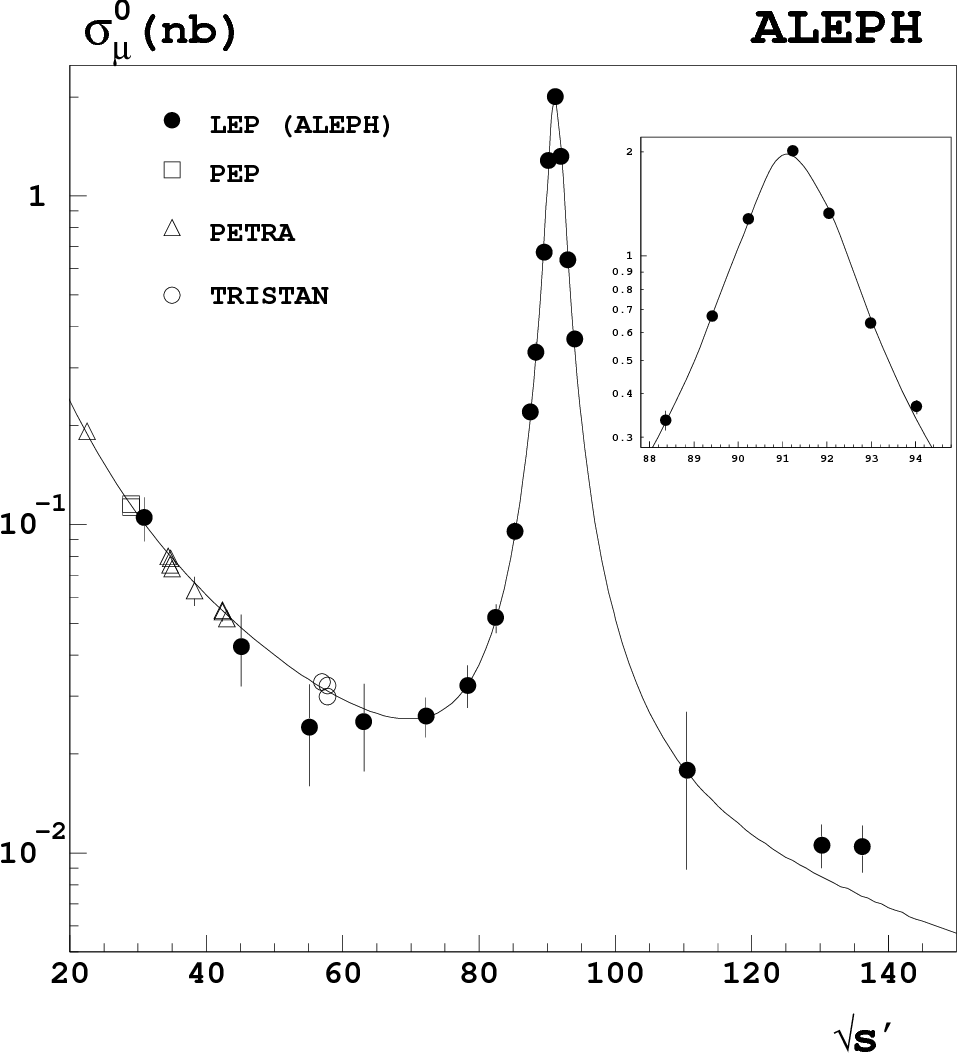
\includegraphics[width=\textwidth]{src/z-resonance.png}
    \end{minipage}
    \hfill
    \begin{minipage}{0.48\textwidth}
        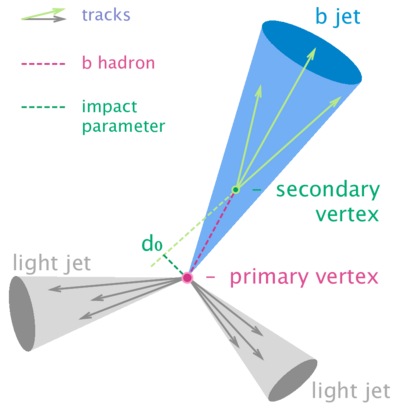
\includegraphics[width=\textwidth]{src/b-tagging.png}
    \end{minipage}
    \caption{(1) The Z boson mass veto. (2) B-tagging.}
    \label{fig:z-veto}
\end{figure}

\subsection{Top Mass Reconstruction Issue}
\textbf{Problem.} (Top mass in step 0 and step 8.)
Step 0 either uses the theory value ($m_t = 172.5 \, \text{GeV}$) or uses massless particles.
Step 8 involves the reconstruction of the top quark mass and lepton masses from the selected events.
The problem is that reconstructed masses from step 8 may have a distribution that is not physical. See \verb|02262025-step8mass.ipynb|. \followup

\section{Bell Test from Spin Correlation}

\subsection{Bell's Inequality, Derivation and Background}

The story begins with the EPR paradox raised in \autocite{EPR1935}, questioning quantum mechanics's consistency with locality principle. Bell's inequality \autocite{bellEPR1964} provides a necessary condition for a quantum two spin-1/2 particle system to admit a \textit{local hidden variable} model. 

Consider the following correlation function
\[
E(a, b)=\int d \lambda p(\lambda) A(a, \lambda) B(b, \lambda),
\]
where $A(a, \lambda)$ and $B(b, \lambda)$ are the outcomes of measurements of spin components $a$ and $b$ on the two particles, respectively. The hidden variable $\lambda$ is distributed according to $p(\lambda)$. In the EPR state, we have perfect anti-correlation, $A(a, \lambda) = - B(a, \lambda)$. Thus,
\begin{align*}
    E(a,b) - E(a, c) 
    &= \int d \lambda p(\lambda) (- A(a, \lambda) A(b, \lambda)) - (- A(a, \lambda) A(c, \lambda)) \\
    &= \int d \lambda p(\lambda) A(a, \lambda) A(b, \lambda) (-1 + A(b, \lambda) A(c, \lambda)) \\
    &\leq \int d \lambda p(\lambda) (1 - A(b, \lambda) A(c, \lambda)) \\
    &= 1 + E(b, c).
\end{align*}
Where, in the inequality we used $A(a, \lambda) A(b, \lambda) \geq -1$ and $(-1 + A(b, \lambda) A(c, \lambda)) \leq 0$. By symmetry between $b, c$ we have

\begin{tcolorbox}[breakable,colback=cyan!10,title=Bell's Inequality]
    \[
|E(a, b)+E(a, c)| \leq 1+E(b, c)
    .\]
    \rule{\linewidth}{0.1em}
    \begin{enumerate}[leftmargin=!,labelindent=!,itemindent=-15pt]
        \item Context: In Bell's 1935 paper, he showed that this inequality is obeyed by any local hidden variable theory. One can find quantum states that violate this inequality, such as the EPR state. This matters because it provides a testable criterion for the violation of local realism.
        \item Symbols and definitions: $E(a,b)$ is the correlation function between the outcomes of measurements of spin components $a$ and $b$ on the two particles, according to the hidden variable $\lambda$. $p(\lambda)$ is the probability distribution of the hidden variable.
        \item Derivation: See above.
        \item Intuition:
    \end{enumerate}
\end{tcolorbox}

Bell's result, although gives a necessary condition for local hidden variable theory, is not directly testable because . In 1969, Clauser, Horne, Shimony, and Holt (CHSH) \autocite{clauserProposedExperiment1969,clauserExperimentalConsequences1974} proposed a testable inequality, now called the Bell-CHSH inequality. They considered a wider class of theories, the \textit{objective local theories} (objective and local).
They addressed the issue of non-ideal detectors and the detection efficiency. The new inequality reads

\begin{tcolorbox}[breakable,colback=cyan!10,title=Bell-CHSH Inequality]
    \[
    -1 \leq p(a, b) - p(a, b') + p(a', b) + p(a', b') - p(a', \cdot) - p(\cdot, b) \leq 0
    .\]
    As a consequence,
    \[
    |p(a, b) - p(a, b') + p(a', b) + p(a', b')| \leq 2
    .\]
    This is sometimes written in modern notation as
    \[
\left|\left\langle\mathcal{B}_{\mathrm{CHSH}}\right\rangle_{\varrho}\right| \leq 2,
\]
    where
    \[
\mathcal{B}_{\mathrm{CHSH}}=\hat{\boldsymbol{a}} \cdot \boldsymbol{\sigma} \otimes\left(\hat{\boldsymbol{b}}+\hat{\boldsymbol{b}}^{\prime}\right) \cdot \boldsymbol{\sigma}+\hat{\boldsymbol{a}}^{\prime} \cdot \boldsymbol{\sigma} \otimes\left(\hat{\boldsymbol{b}}-\hat{\boldsymbol{b}}^{\prime}\right) \cdot \boldsymbol{\sigma}.
\]
    \rule{\linewidth}{0.1em}
    \begin{enumerate}[leftmargin=!,labelindent=!,itemindent=-15pt]
        \item Context: A generalization of Bell's inequality that is experimentally testable. This inequality strictly implies Bell's inequality. However, the technique used in proving Bell's can be adapted to prove this one, as remarked in \autocite[eqn.~B7]{clauserProposedExperiment1969}.
        \item Symbols and definitions: $p(a, b)$ is the probability of both particles having spin up when measured along $a$ and $b$. $p(a, \cdot)$ is the probability of the first particle having spin up when measured along $a$. 
        
        In the modern notation, $\mathcal{B}_{\mathrm{CHSH}}$ is called the \textit{Bell observable}, and $\varrho$ is the density matrix of the two-particle system. $\hat{\boldsymbol{a}}, \hat{\boldsymbol{b}}, \hat{\boldsymbol{b}}^{\prime}, \hat{\boldsymbol{a}}^{\prime}$ are unit vectors in $\mathbb{R}^3$, the directions of the measurement axes. 
        \item Derivation: Start with the below lemma. Take $x_1 x_2 = p(\lambda, a, b)$, etc. (this is possible by locality assumption), and $X = Y = 1$. Then integrate over $\lambda$.
        \item Intuition:
    \end{enumerate}
\end{tcolorbox}
\begin{lemma}
    For $0 \le x_1, x_2 \le X$ and $0 \le y_1, y_2 \le Y$, define $U = x_1 y_1 - x_1 y_2 + x_2 y_1 + x_2 y_2 - Y x_2 - X y_1$. Then $-X Y \le U \le 0$.
\end{lemma}
\begin{proof}
    Direct case analysis. We omit it here. Still available in handwritten notes. 
\end{proof}
\followup Mathematical understanding of such inequalities and relation to convexity can be explored.

Now, if we explicitly write out the density matrix for a system of two spin-1/2 particles, 
\[
\rho = \frac{1}{4} \left(\mathbb{1} \otimes \mathbb{1} + \vec a \cdot \bm \sigma \otimes \mathbb{1} + \mathbb{1} \otimes \vec b \cdot \bm \sigma + \sum_{i,j} C_{ij} \sigma_i \otimes \sigma_j \right),
\]
we note that the probabilities are given by $p(a, b) = a^T C b$, etc. The Bell-CHSH inequality can then be written as
\[
|a^T C (b - b') + a'^T C (b + b')| \le 2.
\]

We have seen that the inequality only depends on the spin correlation matrix $C$. However, to do experiment with this inequality, we need to optimize the measurement axes $\vec a, \vec a', \vec b, \vec b'$. Alternative, we can find some criteria which guarantees existence of such choices of axes that violate the inequality. A necessary and sufficient condition for the violation of Bell's inequality in terms of the correlatin matrix $C$ is given by \autocite{horodeckiViolatingBell1995}.


\begin{tcolorbox}[breakable,colback=cyan!10,title=Bell Inequality Violation]
    The Bell-CHSH inequality
    \[
        \left|\left\langle A_{1} B_{1}\right\rangle+\left\langle A_{1} B_{2}\right\rangle+\left\langle A_{2} B_{1}\right\rangle-\left\langle A_{2} B_{2}\right\rangle\right| \leq 2
    \], or equivalently
    \[
    \left|\vec{a} \cdot C\left(\vec{b}-\vec{b^{\prime}}\right)+\vec{a^{\prime}} \cdot C\left(\vec{b}+\vec{b^{\prime}}\right)\right| \leq 2 \qquad \left|\left\langle\mathcal{B}_{\mathrm{CHSH}}\right\rangle_\varrho\right| \leq 2.
    \]
    is violated if and only if
    \[
        \lambda+\lambda^{\prime}>1
    .\]
    In particular,
    \[
\max _{a, a^{\prime}, b, b^{\prime}}\left|\vec{a} \cdot C\left(\vec{b}-\vec{b^{\prime}}\right)+\vec{a^{\prime}} \cdot C\left(\vec{b}+\vec{b^{\prime}}\right)\right|=2 \sqrt{\lambda+\lambda^{\prime}}.
\]
    \rule{\linewidth}{0.1em}
    \begin{enumerate}[leftmargin=!,labelindent=!,itemindent=-15pt]
        \item Context: This gives a necessary and sufficient condition for the violation of Bell's inequality. This matters because we want experimentally testable criteria for the violation of Bell's inequality. One class of such criteria is spin correlation measurements. 
        \item Symbols and definitions: $\lambda$ and $\lambda'$ are the first two largest eigenvalues of the symmetric positive-definite matrix $M = C^T C$, where $C$ is the correlation matrix of the two-particle system.
        \item Derivation: See \autocite[eqn.~6-9]{horodeckiViolatingBell1995}. The same paper also cites the general upper bound $\left|\left\langle\mathcal{B}_{\mathrm{CHSH}}\right\rangle_\varrho\right| \leq 2 \sqrt{2}$ under QM.
        \item Intuition: \followup Get this from derivation.
    \end{enumerate}
\end{tcolorbox}
However, this approach still has limitations. Computing the eigenvalues of $M$ requires fullly determining the correlation matrix $C$, which is prune to experimental errors. Hence, we develop more conservative criteria for Bell violation, see \autocite[eqn.~15-17]{aguilar-saavedraImprovedTests2022}. We choose specific $\vec a$ and $\vec b$, in order to obtain a stronger condition that only involves the diagonal elements of $C$. To this end, pick $a = (1,0,0)^T, a' = (0,1,0)^T, b = \pm(1,1,0)^T/\sqrt{2}, b' = \pm (-1, 1, 0)^T/\sqrt{2}$. Then we have
\[
\left|C_{1 1} \pm C_{2 2}\right|>\sqrt{2}.
\]
Permuting the axes, we get in general
\begin{tcolorbox}[breakable,colback=cyan!10,title=Bell Inequality Violation]
    A sufficient condition for the violation of the Bell-CHSH inequality is
\begin{equation}
    \label{eq:bell-violation-CiiCjj}
    \left|C_{i i} \pm C_{j j}\right|>\sqrt{2}.
\end{equation}
    \rule{\linewidth}{0.1em}
    \begin{enumerate}[leftmargin=!,labelindent=!,itemindent=-15pt]
        \item Context: The eigenvalue condition is neat, but we want something experimentally simpler.
        \item Symbols and definitions: $C_{ii}$ and $C_{jj}$ are the diagonal elements of the correlation matrix $C$, with respect to any orthonormal basis.
        \item Derivation: See above and below.
        \item Intuition: 
    \end{enumerate}
\end{tcolorbox}

\begin{proof}
One can give a mathematical argument using the eigenvalue interlacing theorem. Assume $C$ is symmetric (which is in practice a very good approximation).
Write $\lambda_1$ and $\lambda_2$ for the largest two eigenvalues of $M = C^T C$.
Let $\Pi$ be the operator that sends a square matrix to its principle submatrix taking away the last row and last column. Use the fact that for a 2x2 symmetic matrix, $\operatorname{Tr } A^2 = \nu_1^2 + \nu_2^2$.
\begin{align*}
    \lambda_1 + \lambda_2 
    &\geq \mu_1^2 + \mu_2^2 = \operatorname{Tr } \Pi C^2 = (C^2)_{11} + (C^2)_{22} \\
    &\geq \operatorname{Tr } (\Pi C) ^2 \\
    &= \operatorname{Tr } \begin{pmatrix}
        C_{11} & C_{12} \\
        C_{21} & C_{22}
    \end{pmatrix}^2\\
    &= C_{11}^2 + C_{22}^2 + 2 C_{12}^2 \\
    &\geq C_{11}^2 + C_{22}^2 \\
    &\geq (C_{11} \pm C_{22})^2/2
\end{align*}
The first inequality is the eigenvalue interlacing theorem. The last inequality is the arithmetic-geometric mean inequality.
To justify the first inequality:
\begin{align*}
    \operatorname{Tr } \Pi C^2
        &= \operatorname{Tr } \begin{pmatrix}
            \Pi C & \vrule & Y \\
            \hline
            Y^T & \vrule & C_{33}
        \end{pmatrix}^2 \\
        &= \operatorname{Tr }(\Pi C)^2 + \operatorname{Tr }(2 Y Y^T) + C_{33}^2\\
        &\geq \operatorname{Tr }(\Pi C)^2
\end{align*}
The proof could be done using direct computation, without an eigenvalue argument. I just like the eigenvalue argument because it is more fancy and beautiful.
\end{proof}


\section{Top quark tomography}
\subsection{Reference Frames}
We consider three frames that are related by rotation-free boosts:
\begin{enumerate}
    \item The lab frame.
    \item The pp COM frame.
    \item The $t$/$\bar t$ rest frame.
\end{enumerate}

\subsection{Angular Distribution}
See \autocite[Sect.~4.2]{bernreutherSetTop2015}. 

We analyze $t \bar{t}$ production at the LHC and subsequent decay into dileptonic final states,
\[
p p \rightarrow t+\bar{t}+X \rightarrow \ell^{+} \ell^{\prime-}+\text { jets }+E_T^{\text {miss }}
\]
and into lepton plus jets final states,
\[
\begin{aligned}
& p p \rightarrow t+\bar{t}+X \rightarrow \ell^{+}+\text {jets }+E_T^{\mathrm{miss}} \\
& p p \rightarrow t+\bar{t}+X \rightarrow \ell^{-}+\text {jets }+E_T^{\mathrm{miss}}
\end{aligned}.
\]
Dileptonic decay is shown in Figure~\ref{fig:ttbar-dilepton}. We have the following 
\begin{tcolorbox}[breakable,colback=cyan!10,title=Angular distribution]
    \[
\frac{1}{\sigma} \frac{d \sigma}{d \Omega_{+} d \Omega_{-}}=\frac{1}{(4 \pi)^2}\left(1+\mathbf{B}_1^{\prime} \cdot \hat{\ell}_{+}+\mathbf{B}_2^{\prime} \cdot \hat{\ell}_{-}-\hat{\ell}_{+} \cdot C^{\prime} \cdot \hat{\ell}_{-}\right)
    .\]
    \rule{\linewidth}{0.1em}
    \begin{enumerate}[leftmargin=!,labelindent=!,itemindent=-15pt]
        \item Context: Describes the angular distribution of the two leptons in the dileptonic decay of $t \bar t$. The state parameters $\mathbf{B}_1^{\prime}, \mathbf{B}_2^{\prime}$ and $C^{\prime}$ contain information from $t\bar t$ production density matrix and $t$ and $\bar t$ decay density matrices. Those density matrices are computed from SM or NP models. Being able to tell the difference between SM and NP is one motivation for this measurement.
        
        \item Symbols and definitions:
        $d \Omega=d \cos \theta d \phi$. 
        The unit vectors $\hat{\ell}_{+}, \hat{\ell}_{-}$, depending on $\Omega_+$ and $\Omega_-$, are the $\ell^{+}$and $\ell^{\prime-}$ directions of flight in the $t$ and $\bar{t}$ rest frames, respectively, which are reached from the $t \bar{t}$ ZMF by rotation-free boosts.
        $(\theta_+, \phi_+)$ and $(\theta_-, \phi_-)$ are the azimuthal and polar angles of the $\hat \ell^+$ and $\hat \ell^-$ directions.

        The \textit{production plane} is the plane orthogonal to the beam axis and containing the $t$ and $\bar{t}$ momenta. The \textit{azimuthal angle} is the angle between the production plane and the $\hat \ell_\pm$ direction. The \textit{polar angle} is the angle between $\hat z$ axis and the $\hat \ell_\pm$ in the COM frame.

        $B_1$ and $B_2$ are the Bloch vectors of the two particle mixed state. Note that they are not necessarily unit vectors, since we are in a mixed state. They are actually equal to $B_1^i=P_i \kappa_l$ where $P_i=\left\langle 2 \vec{\mathbf{S}}_t \cdot \hat{i}\right\rangle$, the spin operator. $\kappa_l \in [0,1]$ is a constant very close to 1, the top spin \textit{analyzing power} computed from QCD.

        \item Derivation: This is general form of the angular distribution of two spin-1/2 particles.

        \item Intuition: Compare this to spin density matrix elements of an EPR state. $B_1$ and $B_2$ are the Bloch vectors of the two particles. $C$ is the spin correlation matrix. One can verify that $\bra{\hat \ell_+ \otimes \hat \ell_-} \rho \ket{\hat \ell _+  \otimes \hat \ell _-}$, where $\rho$ is density matrix for EPR system
        \[
        \rho = \frac{1}{4} \left(\mathbb{1} \otimes \mathbb{1} + B_+ \mathbf{\sigma} \otimes \mathbb{1} + B_- \mathbb{1} \otimes \mathbf{\sigma} + C_{ij} \sigma_i \otimes \sigma_j \right),
        \]
        recovers the formula.
    \end{enumerate}
\end{tcolorbox}

Single lepton decay events are degenerate examples of the above decay. Hence we proceed with the dileptonic decay.

Now, we choose a basis and obtain a parametric formula. The basis we shall use is the \textit{helicity basis}, defined at the collision COM frame, and parallel transported to the $t$ and $\bar t$ rest frames. Recall, the helicity basis $(\hat{k}, \hat{n}, \hat{r})$ is defined as follows: \autocite[Fig.~1]{cmsMeasurementTop2019}
\begin{itemize}
    \item $\hat{k}$ is the direction of the $t$ momentum in the COM frame.
    \item $\hat{n}$ orthogonal to the collision plane, i.e. both beam axis and $t$ momentum. Its direction is determined by $\text{sign}(\hat p \cdot k)\hat{p} \times \hat{k}$ where $\hat{p}$ is the beam axis.
    \item $\hat{r} = \hat{k} \times \hat{n}$.
\end{itemize}
Though we bear in mind that the helicity is practically considered always, we shall work with a general basis in the calculations below. Take two reference axis $\mathbf{a}\neq\mathbf{b}$ in the COM frame. We abuse notation and denote the parallel transported vectors in the $t$ and $\bar t$ rest frames by the same symbols. 

We consider the polar and azimuthal angles w.r.t. $\mathbf{a}$ and $\mathbf{b}$, denoted by $\theta_+, \phi_+$ and $\theta_-, \phi_-$, respectively. In particular, $\cos \theta_+ = \hat{\ell}_+ \cdot \mathbf{a}$ and $\cos \theta_- = \hat{\ell}_- \cdot \mathbf{b}$.
(Recall, polar angle is the angle between the vector and the polar axis.) The angular distribution is then
\[
\frac{1}{\sigma} \frac{d \sigma}{d \cos \theta_+ d\cos\theta_- d \phi_+ d \phi_-}=\frac{1}{(4 \pi)^2}\left(1+\mathbf{B}_1^{\prime} \cdot \hat{\ell}_{+}+\mathbf{B}_2^{\prime} \cdot \hat{\ell}_{-}-\hat{\ell}_{+} \cdot C^{\prime} \cdot \hat{\ell}_{-}\right)
\]
Integrate over azimuthal angles, we have, for example,
\[
    \frac{1}{(4 \pi)^2}\int_0^{2 \pi} \int_0^{2 \pi}\mathbf{B}_1^{\prime} \cdot \hat{\ell}_{+}( \theta_+, \phi_+) d \phi_+ d \phi_- 
    = \frac{1}{4} \mathbf{B}_1^{\prime} \cdot \mathbf{a} \cos \theta_+.
\]
To see this, split $\mathbf{B}_1^{\prime}$ into components parallel and orthogonal to $\mathbf{a}$. Write $B_1 = \mathbf{B}_1^{\prime} \cdot \mathbf{a}$ and similar for $B_2$. Our angular distribution becomes
\[
\frac{1}{\sigma} \frac{d \sigma}{d \cos \theta_{+} d \cos \theta_{-}}=\frac{1}{4}\left(1+B_1 \cos \theta_{+}+B_2 \cos \theta_{-}-C \cos \theta_{+} \cos \theta_{-}\right) .
\]
Here, $B_1 = \mathbf{B}_1^{\prime} \cdot \mathbf{a} =\left\langle 2 \vec{\mathbf{S}}_t \cdot \mathbf{a}\right\rangle \kappa_l $. Make some comments:
\begin{itemize}
    \item We choose the sign in front of $C$ so that, when there is no acceptance cut,
    \[
C(\hat{\mathbf{a}}, \hat{\mathbf{b}})=\kappa_{\ell}^2 \frac{\sigma(\uparrow \uparrow)+\sigma(\downarrow \downarrow)-\sigma(\uparrow \downarrow)-\sigma(\downarrow \uparrow)}{\sigma(\uparrow \uparrow)+\sigma(\downarrow \downarrow)+\sigma(\uparrow \downarrow)+\sigma(\downarrow \uparrow)}
\]
    the ratio is the \textit{double spin asymmetry}, a measure of spin correlation.
    \item In a CP-invariant theory, for choices $\mathbf{a} = - \mathbf{b}$, we have $B_1 = B_2$.
\end{itemize}
We try to further simplify the expression by producing one-dimensional distributions. Define
\[
\xi=\cos \theta_{+} \cos \theta_{-}
\]
and insert $1=\int d \xi \delta\left(\xi-\cos \theta_{+} \cos \theta_{-}\right)$ into the angular distribution. Integrate over $d\theta_+ d\theta_-$, we get
\[
\frac{1}{\sigma} \frac{d \sigma}{d \xi}=\frac{1}{2}(1-C \xi) \ln \left(\frac{1}{|\xi|}\right).
\]
Integrating over $d\theta_\pm$, we get
\[
\frac{1}{\sigma} \frac{d \sigma}{d \cos \theta_{ \pm}}=\frac{1}{2}\left(1+B_{1,2} \cos \theta_{ \pm}\right).
\]
Similarly, we obtain
\[
\begin{aligned}
\frac{1}{\sigma} \frac{d \sigma}{d x_{ \pm}} & =\frac{1}{2}\left(1-\frac{C_{i j} \pm C_{j i}}{2} x_{ \pm}\right) \cos ^{-1}\left|x_{ \pm}\right| \\
x_{ \pm}^{i j} & =\cos \theta_1^i \cos \theta_2^j \pm \cos \theta_1^j \cos \theta_2^i .
\end{aligned}
\]
Similarly, we can obtain another convenient observable:
\[
\begin{aligned}
\frac{1}{\sigma} \frac{d \sigma}{d \cos \varphi}&=\frac{1}{2}(1-D \cos \varphi)
\\
\cos \varphi &= \hat \ell_1 \cdot \hat \ell_2 \\
D&=-\operatorname{Tr}[C] / 3=-\left(C_{k k}+C_{r r}+C_{n n}\right) / 3 .
\end{aligned}
\]
Note, $\hat \ell_1$ and $\hat \ell_2$ are in their respective top and anti-top rest frames.

We summarize the observables in the following table:
\begin{center}
    \begin{longtable}{|c|c|c|}
        \hline
        Observable & Measured Coefficient & Symmetries \\
        \hline
        $\cos \theta_+^k$ & $B_1^k$ & P-odd, CP-even \\
        $\cos \theta_-^k$ & $B_2^k$ & P-odd, CP-even \\
        $\cos \theta_+^r$ & $B_1^r$ & P-odd, CP-even \\
        $\cos \theta_-^r$ & $B_2^r$ & P-odd, CP-even \\
        $\cos \theta_+^n$ & $B_1^n$ & P-even, CP-even \\
        $\cos \theta_-^n$ & $B_2^n$ & P-even, CP-even \\
        \hline
        $\xi^{kk}$ & $C^{kk}$ & P-even, CP-even \\
        $\xi^{rr}$ & $C^{rr}$ & P-even, CP-even \\
        $\xi^{nn}$ & $C^{nn}$ & P-even, CP-even \\
        \hline
        $x_+^{rk}$ & $C^{rk} + C^{kr}$ & P-even, CP-even \\
        $x_-^{rk}$ & $C^{rk} - C^{kr}$ & P-even, CP-odd \\
        $x_+^{nr}$ & $C^{nr} + C^{rn}$ & P-odd, CP-even \\
        $x_-^{nr}$ & $C^{nr} - C^{rn}$ & P-odd, CP-odd \\
        $x_+^{nk}$ & $C^{nk} + C^{kn}$ & P-odd, CP-even \\
        $x_-^{nk}$ & $C^{nk} - C^{kn}$ & P-odd, CP-odd \\
        \hline
        $\cos \varphi$ & $D$ & P-even, CP-even \\
        \hline
    \end{longtable}
    \captionof{table}{Summary of observable quantities measuring spin correlations in $t\bar{t}$ production, their corresponding coefficients, and their transformation properties under parity (P) and charge-parity (CP) symmetries. Superscripts $k, r, n$ denote the choice of $\mathbf{a}$ and $\mathbf{b}$ in definition of the observables.}
\end{center}
\begin{remark}
    Parity symmetry (P) is the transformation $\mathbf{x} \mapsto -\mathbf{x}$, while charge-parity symmetry (CP) is the transformation $\mathbf{x} \mapsto -\mathbf{x}$ and exchanging top and anti top. \followup We see that $B^n$ is P-even and $B^{k}, B^{r}$ are P-odd, while all $B$'s are CP-even. Diagonal elements of $C$ are P- and CP-even, whereas off-diagonal elements are more complicated. 

    Those symmetry considerations seems to have guided our choice of $\mathbf{a}$ and $\mathbf{b}$ as specific combinations of the helicity basis vectors. \followup
\end{remark}

For reference, see \autocite[Sect.~2]{cmsMeasurementTop2019}. 

\begin{tcolorbox}[breakable,colback=red!10, title=Remaining Questions]
\begin{itemize}
    \item I still don't understand \autocite[eqn.~3]{cmsMeasurementTop2019} and the symmetry discussion that follows. 
    \item In \autocite[Sect.~3]{quirosProtonProtonCollisions2024}, antisymmetry is computed analytically for each Measured Coefficient. How is this used? In \autocite[eqn.~11]{cmsMeasurementTop2019} the antisymmetry is only computed for some extra lab frame observables.
    \item Is $\cos \theta_+$ and $\cos \theta_-$ computed both in top helicity basis, or one in top and one in anti-top helicity basis? {\color{purple!5} - There is only one helicity basis, defined w.r.t. the top direction.}
\end{itemize} 
\end{tcolorbox}

\subsection{Tomography from Angular Distributions}
    
Next, to extract the parameters $B_{1, 2}$ and $C$ ($3 + 3 + 9 = 15$ entries in total), we compute the \textit{asymmetry} of the angular distribution. We refer to \autocite[eqn.~(2.21)]{quirosProtonProtonCollisions2024}. For any distribution of the form $g(\Lambda ; \lambda)=\frac{1}{\sigma} \frac{\mathrm{~d} \sigma}{\mathrm{~d} \Lambda}$, where the variable $\Lambda \in[-1,1]$, the asymmetry is defined as
\[
A_\lambda=\frac{\int_0^1 d \Lambda g(\Lambda ; \lambda)-\int_{-1}^0 d \Lambda g(\Lambda ; \lambda)}{\int_{-1}^1 d \Lambda g(\Lambda ; \lambda)}=\frac{N(\Lambda>0)-N(\Lambda<0)}{N(\Lambda>0)+N(\Lambda<0)}
\]
On one hand, the asymmetry is computed analytically from each distribution $g(\Lambda ; \lambda)$, yielding a relation of the form $\lambda=a_\lambda A_\lambda$. On the other hand, the asymmetry is measured experimentally. This gives dierct access to the parameters $\lambda$.

\begin{example}
    Consider the parameter $B_1^k$ for example, we simply write $B$. The asymmetry is computed from the distribution
    \[
        \frac{1}{\sigma} \frac{d \sigma}{d \cos \theta} = \frac{1}{2} (1 + B \cos \theta).
    \]
    Here $\cos \theta$ ranges from $-1$ to $1$. We integrate the right hand side over $-1$ to $0$ and $0$ to $1$ to get the asymmetry. We have
    \[
        \int_0^1 d \cos \theta \frac{1}{2} (1 + B \cos \theta)  = \frac{1}{2} + \frac{B}{4},
    \]
    and
    \[
        \int_{-1}^0 d \cos \theta \frac{1}{2} (1 + B \cos \theta)  = \frac{1}{2} - \frac{B}{4},
    \]
    Thus, we get $A_B = B/2$, i.e. $B = 2 A_B$, i.e. $a_B = 2$.
\end{example}

The following table summarizes the ratios $a_\lambda$ for each parameter $\lambda$.
\begin{center}
\begin{tabular}{|c|c|c|c|c|}
    \hline$\lambda$ & $B_{1,2}^i$ & $C_{i j}$ & $C_{i j} \pm C_{j i}$ & $D$ \\
    \hline$a_\lambda$ & $2$ & $-4$ & $-16 / \pi$ & $-2$ \\
    \hline
\end{tabular}
\end{center}



\newpage
\printbibliography

\end{document}
